Researchers found that advances in the field of deep learning -- a broad family of methods based on artificial neural networks -- can be used to enhance the classical RL algorithms.
This led to the expansion of the field, marking the birth of \textbf{deep reinforcement learning (deep RL)}.

Classic RL assumes that the state space is finite and can be modeled in a tabular manner.
However, we seldom encounter real-world, interesting problems where this assumption holds.
Deep RL is an open field striving to solve \emph{more complex} problems than classical methods allow.
This is done through the ability of functional approximators to model high-dimensional spaces.

The field has recently surged, after a series of new algorithms and succesful applications were published.
In this chapter, we try to give an overview of the main methods of learning but mainly focus on developing \emph{Mnih et al.'s \textbf{DQN} (2013)} \cite{atari-dqn}.

In Section \ref{section:convnets}, we present \textbf{convolutional neural networks}, a class of artificial neural networks which became the foundation of multiple algorithms in deep RL.

Section \ref{section:dqn} covers using neural networks (called deep Q-networks in the paper \cite{atari-dqn}) as approximators in Q-learning in order to build autonomous agents for complex model-free environments.

The rest of the chapter (Sections \ref{section:policy-opt} and \ref{section:actor-critic}) deals with alternative strategies for doing (deep) model-free control, namely \textbf{policy optimization} and \textbf{actor-critic} methods respectively.

\clearpage

\subsection{Convolutional Neural Networks (ConvNets)} \label{section:convnets}
\textbf{Convolutional neural networks} (often shortened as ConvNets or CNNs) are a specific type of artificial neural network for processing data that has a known grid-like topology \cite{Goodfellow-et-al-2016}.

ConvNets exploit the \textbf{spatial nature} of the data.
This property makes them especially useful over a vast spectrum of problems, such as image classification, audio signal processing, analyzing financial time-series etc.
Among those, image classification tasks are the primary reason for the architecture's popularity.

The \textbf{origin} of convolutional networks can be traced back to Kunihiko Fukushima's \emph{neocognitron} (1979).
Kunihiko’s design \cite{neocognitron-paper} was itself inspired by earlier breakthroughs in neuroscience -- namely studies of the visual cortex of mammals (Hubel \& Wiesel, 1959).
LeCun et al. (1989) further improved this model by introducting backpropagation training, which set the standard for today’s architectures.

\subsubsection{Overview}
A convolutional network contains at least one convolutional layer in its structure.
A typical convolutional layer (represented in Figure \ref{fig:conv-layer}) is composed of three stages \cite{Goodfellow-et-al-2016}:
\begin{enumerate}
    \item The \textbf{convolution stage} convolves the input data with a filter (kernel), which results in a set of linear activations.
    The kernel is the learned element, i.e. we learn the weights of the kernel as we would learn the weights of a linear layer.
    \item The \textbf{detector stage} pipes each linear activation from the convolution layer thorugh a non-linear activation function (e.g. ReLU \footnotemark)
    \item The \textbf{pooling stage} is an optional stage which reduces the output size by computing summary statistics over the data.
\end{enumerate}
\footnotetext{standing for \emph{rectified linear unit}, it is commonly used as an activation function in neural networks. In its classic form, it can be expressed as $f(x) = max(0, x)$.}

\begin{figure}[h]
    \centering
    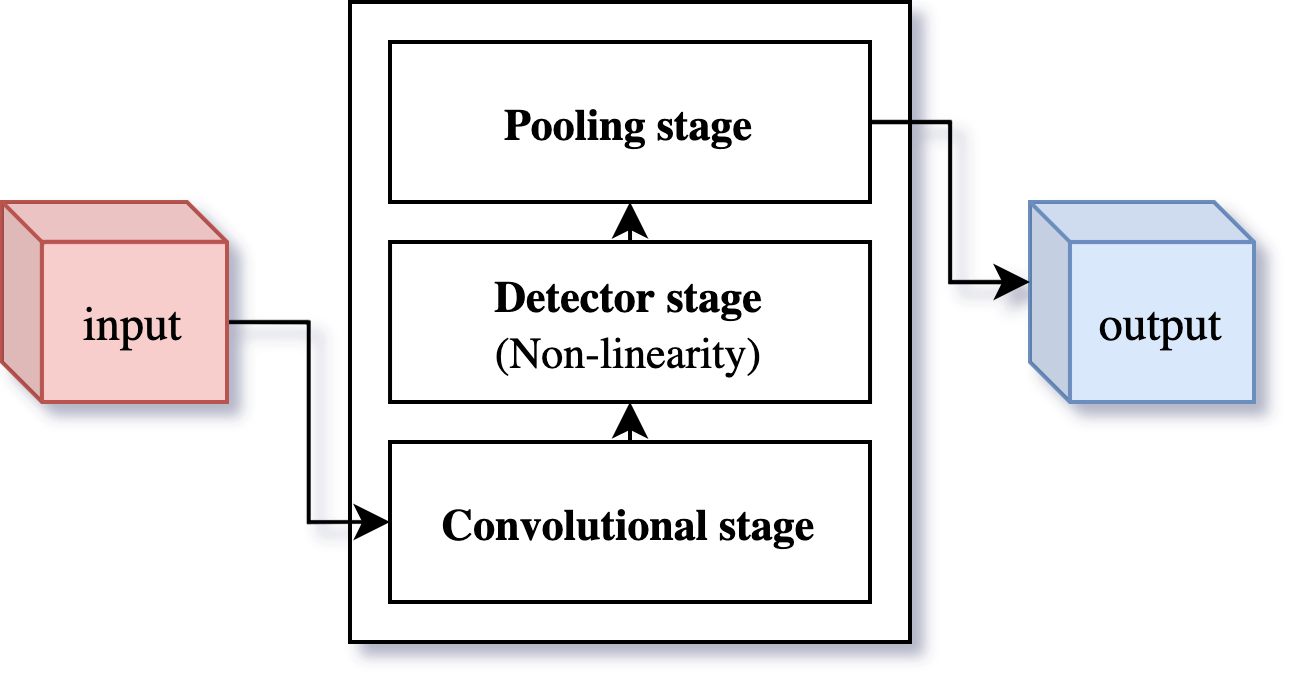
\includegraphics[width=0.7\textwidth]{conv-layer-structure.png}
    \caption{A schematic of a convolutional layer.}
    \label{fig:conv-layer}
\end{figure}

In this section, we consider the \textbf{input} and \textbf{output data} to be 3D tensors, consisting of a spatial dimension (width and height) and a depth dimension.
Visualizing this process with images in mind is particularly helpful to understanding.
The spatial dimensions map exactly to the width and height of an image, and each color channel can be considered a separate depth level.


\subsubsection{The Convolutional Stage}
This stage performs the convolution operation which is the most computationally demanding procedure of the layer.
The output from this stage is a \textbf{feature map} of the input, which is then passed as linear activation to the detector stage, likewise to fully-connected feedforward networks.

This \textbf{operation} consists of sliding a \emph{kernel} over the input.
At every step, we compute the dot product between the kernel and the volume of input it currently overlaps.
The \textbf{kernel} (or filter) is a tensor of adjustable weights, which is small relative to the image's spatial dimentions but must cover the entire depth of the image.
The effects of the convolutional stage are determined by a number of hyperparameters: depth, stride and padding.

A convolutional stage can learn multiple independent kernels.
The number of kernels is given by the \textbf{depth} hyperparameter.
It is conveniently called such because it corresponds to the depth of the output of this stage.
A \textbf{depth column} (or fibre) \cite{stanford-convnets} is a set of neurons ``looking'' to the same region in the input (where each neuron corresponds to a different kernel) .

The \textbf{stride} specifies the distance which we slide the kernel with over the input at each step.
Some models provide separate stride parameters for each axis (horizontal and vertical) \cite{Goodfellow-et-al-2016}.

\textbf{Zero-padding} (or simply padding) enables padding our input data with zeros along the borders. It is useful for controlling output size, especially in cases where we want to preserve the input size over multiple layers.

\begin{figure}[h]
    \centering
    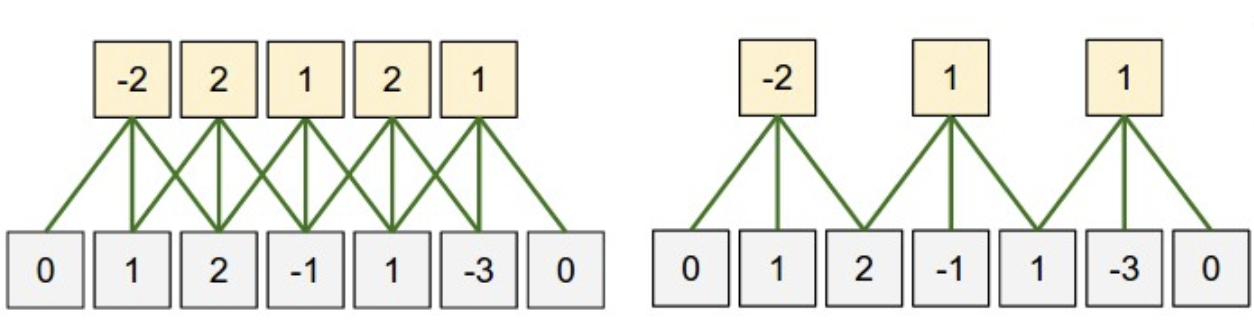
\includegraphics[width=0.6\textwidth]{conv-stride-padding.png}
    \caption{(Left) Using a stride of 1 and a zero-padding of 1 to preserve the original spatial dimensions of the input. (Right) Using a padding of 1 and a stride of 2, which results in fewer output values. (Illustration from \cite{stanford-convnets})}
    \label{fig:conv-stride-padding}
\end{figure}
 
The properties of convolution confer ConvNets a myriad of advantages over fully-connected feedforward neural networks.
This gain in efficiency comes from the assumption that the data has an underlying spatial structure, which can be exploited better by ConvNets than by alternatives.

Typical fully-connected layers relate all their outputs to all their inputs by separate, \emph{independently adjustable} weights.
This requires storing weight matrices as large as the input data itself, rising the computational cost as input size grows.
In contrast, kernels are significantly smaller than the input volume is (in the spatial dimensions).
Kernels are also reused across the entire layer (\textbf{parameter sharing}), resulting in smaller memory requirements.

ConvNets feature \textbf{sparse interactions}, in contrast to the dense interactions of fully-connected layers in which every output is related by a weight to each of the input values.
This boosts learning efficiency by reducing the number of necessary computations.

Learning smaller, shared kernels can be a means of controlling \emph{overfitting} \cite{Goodfellow-et-al-2016}. Moreover, ConvNets can operate on input data of \textbf{varying sizes} without making adjustments to model architecture.


\subsubsection{Pooling}
The \textbf{pooling stage} is an optional stage in the ConvNet architecture which performs a \emph{downsampling} of its inputs.
The role of this stage is to gradually reduce computation (and memory requirements) in the network by reducing the spatial dimension of the data \cite{stanford-convnets}.
It processes output from the convolutional stage by applying a pooling function.

A \textbf{pooling function} computes a summary statistic (e.g. maximum, average, $l^2$-norm etc.) over a neighbourhood of input values \cite{Goodfellow-et-al-2016}.
The pooling stage has a similar operation to the convolutional stage:
a moving window is slided over and across the input data and at each step, the summary is computed.

Each depth slice of the data is processed independently.
An example for a simple but commonly used operation (max pooling) is shown in Figure \ref{fig:maxpooling}.

\begin{figure}[h]
    \centering
    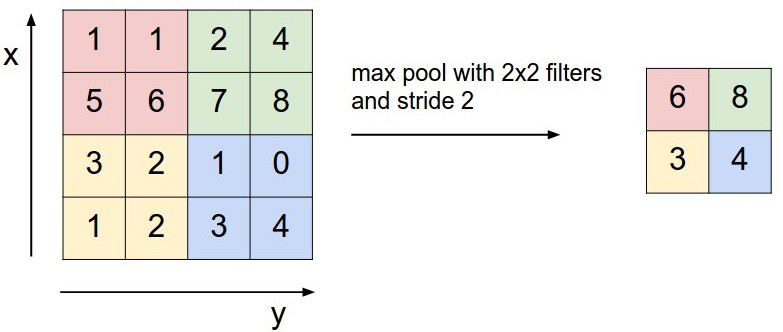
\includegraphics[width=0.8\textwidth]{conv-maxpooling.jpg}
    \caption{Simple example illustrating max pooling (on a single depth level). Illustration from \cite{stanford-convnets}.}
    \label{fig:maxpooling}
\end{figure}

\subsection{Deep Q-Networks (DQN)} \label{section:dqn}
To reiterate our chapter introduction, a key challenge of applying RL to real-world problems is data representation (in the form of policies and value functions).
Real applications require modelling large, high-dimensional problem spaces and hence depend upon functional approximation.

However, functional approximators, whether linear or nonlinear, require ready access to \textbf{features}.
A \textbf{feature} is an independent, measurable property of an observed phenomenon.
Choosing which features of the training data yield the most \emph{relevant} information is a central problem in machine learning.
This is obvious from the perspective of supervised learning, but the same principle applies to RL problem environments.

Most succesful systems (prior to DQN) have relied on \textbf{handcrafted feature sets}, created by experts to capture the problem-relevant information so the RL system does not have to.
Other attempts have relied on \textbf{autoencoders} as a preprocessing step to lower the dimensionality of the observation before feeding it to the agent (used for example in \emph{neural Q-fitting} \cite{neural-q-fitted}).

This section introduces \emph{Mnih et al.}'s \textbf{DQN} \cite{atari-dqn}, a deep model-free learning method that uses \textbf{automatic feature extraction} (is capable of finding an efficient representation directly from interactions with the environment).
The researchers have demonstrated that a DQN agent with the same hyperparameters is able to learn from widely different environments, with no prior knowledge.

The paper benchmarks the agent on 49 video games for the Atari 2600, using the Atari Learning Environment \cite{ale-paper} (a extension layer over an emulator, specially designed to serve as a task environment).
The selection features diverse mechanics and some games require the development of long-term strategies to perform reasonably well at.
The vanilla DQN agent scored better than existing methods (including NEAT\footnotemark) on the vast majority of the games.
\footnotetext{standing for \emph{neuroevolution of augmenting topologies}, a genetic algorithm for generating neural network topologies}
Moreover, it managed a human-like performance at a considerable number of games, according to the evaluation techniques used in the paper.
According to this evaluation, the agent scored highest in \emph{Pong}, \emph{Enduro} and \emph{Breakout}, outperforming expert human players.

\subsubsection{Algorithm}
% Overview of the learning process: how we model the RL problem into a deep learning problem
The algorithm described in the paper is roughly based on \textbf{Q-learning} (described in Section \ref{rl:q-learning}), fitted with deep convolutional networks which approximate the action-value function $Q$, suggestively called \textbf{deep Q-networks}.

% Algorithm specificiation from paper
% Computing the gradients using Q-learning’s update formula
% Defining and optimizing the loss function
% RMSProp (see green paragraph above) 

% This should remain the end paragaph, in order to transition to explanations for experience replay and target networks.
Off-policy learning, bootstrapping (both characteristics of Q-learning) and functional approximation are \textbf{incompatible} at a fundamental level (the three elements comprise the so-called \emph{deadly triad} \cite{rlai}), as the combination fails to converge in theory.
In order to work properly, DQN modifies Q-learning in a few fundamental ways to overcome this incompatibility, by using \textbf{experience replay} and an additional \textbf{target network}.

\subsection{Policy Optimization Methods} \label{section:policy-opt}

\subsection{Actor-Critic Methods} \label{section:actor-critic}
